%!TEX root = ./main.tex

\documentclass[11pt, oneside]{book}

\usepackage[utf8]{inputenc}
\usepackage[english]{babel}

% page layout
\usepackage{float}
\usepackage{ragged2e}
\usepackage{rotating}

% toc renaming
\addto\captionsenglish{
	\renewcommand{\listfigurename}{List of figures}
	\renewcommand{\listtablename}{List of tables}
}
% bib
\usepackage[
backend=bibtex,
style=ieee,
maxbibnames=4,
maxcitenames=4]{biblatex}
\makeatletter
\def\blx@maxline{77}
\makeatother

\usepackage{csquotes}
\usepackage[nottoc]{tocbibind}

\addbibresource{references.bib}

% acro, table, lists etc
\usepackage{acronym}
\usepackage{enumitem}
\usepackage{graphicx}
\usepackage{tabularx}
\usepackage{longtable}
\usepackage{array}
\usepackage{multirow}

\usepackage{lscape}

% formatting
\usepackage{color}


% symbols
\usepackage{eurosym}

% refs
\usepackage{hyperref}
\usepackage{cleveref}

% indent
\usepackage{indentfirst}
\setlength\parindent{24pt}

\hypersetup{
	colorlinks=false, pdfborder={0 0 0},
}

\crefname{lstlisting}{listing}{listings}
\Crefname{lstlisting}{Listing}{Listings}

% listings
\usepackage{listings}

% todo
\usepackage{todonotes}

\lstset{frame=tb,
	language=Java,
	aboveskip=3mm,
	belowskip=3mm,
	showstringspaces=false,
	columns=flexible,
	basicstyle={\small\ttfamily},
	numbers=none,
	numberstyle=\tiny\color{gray},
	keywordstyle=\color{blue},
	commentstyle=\color{dkgreen},
	stringstyle=\color{mauve},
	breaklines=true,
	breakatwhitespace=true,
	tabsize=3
}

\begin{document}

%!TEX root = ./main.tex
\begin{titlepage}
	
    \centering
    
\includegraphics[scale = 0.115]{Pictures/logo.jpg}\\[1.7 cm]	% University Logo
    {\Huge Advanced Software Architecture \par}
    \vspace{1cm}
    {\Large Train ticketing system}

    \vfill
    \justifying
    {\large \begin{itemize}[label={}]
        \item Aida Baxhaku (3242528)
        \item Petar Hariskov (3226735)
        \item Alexandra Matreata (3179265)
        \item Eric Rwemigabo (3040356)
    \end{itemize}}
    
    \vspace{2cm}
    \centering
    {\Large \today \par}
    \vspace{0.1cm}
    {\large version 1.0.0}
\end{titlepage}

\frontmatter

\chapter{Revision history}
\label{chp:rev_his}
%!TEX root = main.tex


%!TEX root = main.tex

\tableofcontents

\listoffigures

\listoftables

\chapter{Glossary}
\label{chp:glos}
%!TEX root = main.tex

\begin{acronym}[]
    \acro{ET}{Easy Ticketing}
    

\end{acronym}

\mainmatter

\chapter{Introduction and goals}
\label{chp:intro}
\section{Introduction}
Traveling by train is one of the most common means of transport in the Netherlands and the Western Europe. The majority of people use trains on a daily basis, to go to school, work, etc. It is quite easy and comfortable, but one common problem, that everyone may relate to is the discomfort of train tickets. The printed tickets might get lost, or a passenger might forget to check in, another one is too late to buy one, etc. 

However, we have come up with an alternative train ticket, which will facilitate the journey of many passengers: \ac{ET}. This is a new, promising and innovative technology that suits practically everyone who owns a smartphone. The idea  behind \ac{ET} is very simple: you download an app in your smartphone, open your personal account and connect it to your favorite payment method, and \ac{ET} will do everything else automatically. 

This means, every train will have beacons, which will connect to the passenger’s phones via  bluetooth, it will check the passenger in,  it will automatically calculate the ticket fee and it will reconnect  when the passenger leaves the train. There will be a beacon per every gateway. The beacon can detect the mobile in a diameter of 20m.

The aim of this new technology is to facilitate the journey of train passangers, and take the ticket purchasing to the next level. We plan to implement \ac{ET} firsly in Groningen and after the initial success the aim of our company is to cover the whole Netherlands. 

In this document we are presenting the architecture of our system. In the next chapters you will be introduced to the Stakeholders of the systems and their concerns, the requirements, functional and non-functional.  In section 3, we will briefly analyze the business context and the benefits that \ac{ET} will brings in terms of business. In section 4, the solution strategy is presented, in terms of our main key drivers. Section 5 outlines the building block view, whereas chapter 6 and 7 introduce the runtime and deployment view. The architecture of our system will be concluded with the design decisions and quality scenarios. 

\section{Quality goals}

The top three goals of the architecture of Easy Ticketing whose fulfillment is of highest importance to the major stakeholders (as agreed between them) are listed below:

\textbf{Security} In our system, we could view the importance of security in two major aspects: Firstly, hackers might hack the system and steal money from the account of the train company and secondly, passengers might find a way to fake their tickets. In both cases, this is unacceptable for our customer under any circumstance. Therefore the system must be designed in such way that potential data leaks, which are in theory inevitable, will not result in access to the main database or create damage to the company.

\textbf{Reliability}  Customers are expected to rely on the functioning of Easy Ticketing. Problems with availability of the service are almost as undesirable as security issues, therefore availability must be taken into account throughout the whole system architecture. Breakdown of the system could lead to financial loss for the company, which is in any case not acceptable.

\textbf{Compatibility} Is an important driver for our system. Passengers may be in possession to different smartphones, which may result in incompatibility with the beacon, incompatible frequencies of bluetooth. It is very important to provide the passengers the possibility to purchase the ticket, for as many phone versions as possible.


\chapter{System scope and context}
\label{chp:syst_context}
This section outlines the main relations between the system and its environment, external systems or entities with which it interacts. The business and technical contexts in which the system will perform as well as different inter-component communication solutions will be presented in this chapter.

\section{Business context}
\label{sec:business_context}
The system focuses on simplifying the management of information related to train traveling and ticket payment for its users. The system will provide an account for each user which will store information regarding travel distance, destinations, payments, etc. This will help both users travelling by train and the companies providing the travelling services by keeping track of all these components in a centralized manner. 

The system will present the user with the choice of making an automated payment for each trip through the connection between the mobile app and the beacon in the train cart. Alternatively, an external payment system will be presented to the user I every train station where they can log in and perform the transaction. 

A second important target for our system will be represented by companies providing travelling services by train, which may include governmental institutions or different private companies.

\section{Business drivers}
This chapter describes the business forces acting on the system: most important revenue streams and costs and give a justification for the system.

\subsection{Revenue streams}
The main revenue stream for the system will consist of the travel service providers. In order to use the Easy Tickting system, they will have to pay a monthly fee which will include storage and maintenance costs. 

Depending on how well the system usage evolves over time, once enough travel service providers decide to use the system, a small monthly fee can be charged to the user as well. Also, the mobile app functionalities can be improved over time and be accessed by the user over a pay-by-use scenario(e.g. check distances travelled over the last period of time, check fees, see a list of possible price reductions for similar journeys).

\subsection{Costs} 
The costs for the system will be divided in two main groups:
\begin{itemize}
	\item \textbf{development costs:} \\
	these costs will be comprised of installation costs(hardware equipment such as beacons and local servers will be installed and configured inside the trains, central server configuration, backup servers configuration) and software development costs(for the mobile application, databases, computational algorithm for fee calculations).
	\item \textbf{maintenance costs:} \\
	maintenance operations will include constant monitoring of the hardrware equipment(remote monitoring and repairs for components inside the trains and a local team for the central server) and a team for additional functionalities(for the mobile app, optimisations of the computational algorithm, etc).
\end{itemize}



\section{Domain model}
\label{sec:domain_model}
Figure \ref{fig:domain_model} outlines the most significant entities taking part in or being used by the Easy Ticketing system. The system components and their interactions are presented alongside the main external entities needed for different functionalities of the system. The figure also introduces the main actors responsible for the use cases presented in chapter \ref{chp:usecases}.

\begin{figure}[H]
	\centering
	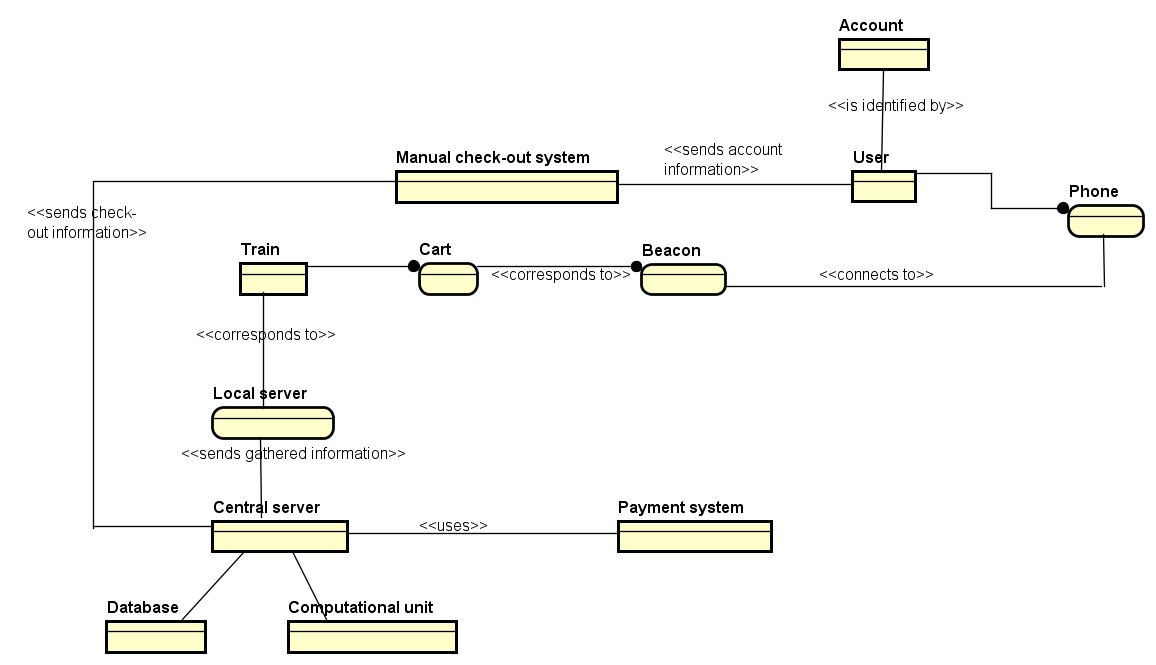
\includegraphics[width=\textwidth]{Pictures/domain_model.png}
	\caption{Domain model}
	\label{fig:domain_model}
\end{figure}

\section{Technical context}
\label{sec:technical_context}
The system will need to perform in a specifically designed technical context consisting of three main environments: a central server collecting all information and performing necessary computations, the setup inside the trains themselves (comprised of beacons and small servers which will collect information per train and send it to the central one every time the train leaves the station) and a login system in each station allowing users to manually check-out of their trip and perform payment.

A set of measures will need to be taken into consideration for the system to be able to operate inside this context by using these different components and environments. These measures will be related to the key attributes required of the system as follows:
\begin{itemize}

\item \textbf{security}: since the system will have access to sensitive information (such as location, financial transactions), every connection between components of the system will need to be secured and trusted. The main connections which will need to be verified each time they are created will be: beacon to mobile application, beacon to server inside the train, small local server to central server. 

\item \textbf{reliability}: for the system to be considered reliable, the main components should be provided with a back-up in case of failure, such as the central server, the beacons in each cart, etc. Also, users should be presented with alternative scenarios in case the main desired activity flow gets interrupted (e.g. possibility to manually check-out of a trip using login system in train station in case of beacon to phone communication being severed)

\item \textbf{compatibility}: the system will need to be compatible with at least the main and most commonly used mobile OS and frequencies 

\end{itemize}

\section{External interfaces}
\label{sec:ext_interfaces}
%!TEX root = main.tex

\begin{table}[H]
  \centering
  \begin{tabularx}{\linewidth}{l|X}
    \textbf{Channel}      & Beacon $\Rightarrow$ Mobile app \\ \hline
    \textbf{Description}  & Beacons detect mobile phones in their proximity having installed the application and initialise a connection.\\ \hline
    \textbf{Connection}   & Bluetooth \\ \hline
    \textbf{Protocol}     & iBeacon \\ \hline
    \textbf{Frequency}    & The train has left a station and a mobile phone is in range of the beacon. \\ \hline
  \end{tabularx}
  \caption{Interface - Beacon to phone}
  \label{tbl:beacon_to_phone}
\end{table}

\begin{table}[H]
	\centering
	\begin{tabularx}{\linewidth}{l|X}
		\textbf{Channel}      & Beacon $\Rightarrow$ Local train server \\ \hline
		\textbf{Description}  & Beacons send information gathered every time a train departs from a station.\\ \hline
		\textbf{Connection}   & Bluetooth \\ \hline
		\textbf{Protocol}     & iBeacon \\ \hline
		\textbf{Frequency}    & The train has left a station. \\ \hline
	\end{tabularx}
	\caption{Interface - Beacon to server}
	\label{tbl:beacon_to_server}
\end{table}

\begin{table}[H]
	\centering
	\begin{tabularx}{\linewidth}{l|X}
		\textbf{Channel}      & Local server $\Rightarrow$ Central server \\ \hline
		\textbf{Description}  & The local server situated inside the train sends information gathered periodically to the central server if an internet connection is possible.\\ \hline
		\textbf{Connection}   & Internet \\ \hline
		\textbf{Protocol}     & UDP \\ \hline
		\textbf{Frequency}    & Once every 20 min or when a connection is possible. \\ \hline
	\end{tabularx}
	\caption{Interface - Local server to central server}
	\label{tbl:local_to_central}
\end{table}

\chapter{Requirements}
\label{chp:requirements}
%!TEX root = main.tex

In this section the main Stakeholders and the functional and non functional requirements of Easy Ticketing will be introduced.

\section{Stakeholders}
The following stakeholders are described along with their concerns. These concerns eventually determine the key drivers of the service.

\subsection{Represented stakeholders}


\textbf{Passengers}  are the direct users of Easy Ticketing. The typical target customer is the traveler who uses the train systems regularly. Passengers are mainly concerned with the reliability and the availability of the system as well as the security often their data and the regular payment of the ticket. If the service is not available then they risk not having a ticket and eventually getting a fine.  Another concern of the passengers could be the incompatibility of their phone with the beacon, which could risk the validity of their ticket.

\textbf{Customers} are the owners of the Easy Ticketing. The typical target are the large train companies, operating in the Netherlands. The companies are mainly concerned with the reliability of the system, since many passengers could end up not paying, given that there is a breakdown of the system. This could result in monetary loss for the company. Another main concern of our customer is the security. If the system is hacked the  company loses money and this is certainly something that the company wants to avoid.

\textbf{Developers and maintenance team} is responsible for building the software part of our system, test and debug it afterwards. They are mainly concerned with the maintainability, testability and portability of the system.

\textbf{Architects} will be the team that will design the system. Their main concern is satisfying the needs of all the stakeholders and finding the best solution. They determine the feasibility of desired properties and functions, and guarantee a satisfactory end-product.


\subsection{Non represented stakeholders}


\textbf{Hardware companies}  are the companies that provide beacons for our system. In our case they are non represented stakeholders, since they do not have much say  


\textbf{Hardware maintenance team} maintains the physical side of the system, in our case beacons and takes care of handling malfunctions.

\textbf{Ticket inspectors} are the employees of the Train companies, that check the passengers, whether they have an available ticket or not. The are mostly concerned with the security and the reliability of the system.

\textbf{Third party payment systems} are companies that provide a paying system for the passengers.  


\section{Key Drivers}


In order to determine the most important key drivers for our system, the stakeholders are required to give points to the key drivers according to what they consider as the most important driver for the system. Since the weight of the decision differs among our stakeholders, they are given different amount of points. The train companies (customer) have 150, the architects have 120, the developer team has 100, and the passengers 80. Considering the distribution of the points, the top 3 will be chosen as key drivers of our system. \cref{tbl:key_drivers} below shows how the different stakeholders used there points.

\begin{table}[H]
  \centering
  \begin{tabularx}{\textwidth}{l|lllllll}
    & \rotatebox[origin=l]{75}{Security} & \rotatebox[origin=l]{75}{Reliability} & \rotatebox[origin=l]{75}{Compatibility}& \rotatebox[origin=l]{75}{Performance} & \rotatebox[origin=l]{75}{Maintainability} & \rotatebox[origin=l]{75}{Scalability} \\ \hline
   
    Train Companies(Customer)    & 50  & 50 & 20 & 30          & 0           & 0      \\
    Architects                   & 50  & 30 & 20 & 20          & 0           & 0      \\
    Developer team               &  0  & 10 & 10 & 20          & 50          & 10     \\
    Passengers                   & 40  & 10 & 30  & 0          & 0           & 0      \\
    Total                & \textbf{140} & \textbf{100}& \textbf{80}  & 70  & 50   & 10    \\
  \end{tabularx}
  \caption{Key driver selection}
  \label{tbl:key_drivers}
\end{table}


\begin{description}[align=left]
  \item[Security] is concerned with the management of possible risks that may affect our system. Since \ac{ET} is working with delicate data which involves payments and bank account records The stakeholders came to the agreement that security is the most important key driver of the system. It is mostly affected by the ability of the system to survive attacks, threats, the algorithms used, etc. The customers(train companies) and passengers are mostly concerned with security. 
  
  \item[Reliability] is measured as the probability that a system will not fail and that it will perform its intended function for a specified time interval. This can be guaranteed by  redundancy, implementing an extra database, increase in resources, implementation of more than a single point of failure for different parts of the system, etc. Passengers are mostly concerned with the reliability of the system as they don't want to risk not having a ticket, while train companies do not want to get any economical loss. 
  
  \item[Compatibility] is the ability of the software to work with other systems. In the case of \ac{ET}, the system should be able to adapt to three different types of the operating system of the smartphones: iOS, Android, Windows. The stakeholders that are mostly concerned with this, are the passangers and the train companies.  

  \item[Maintainability]  is the \cite{web:software} ability of the system to undergo changes with a degree of ease. These changes could impact components, services, features, and interfaces when adding or changing the functionality, fixing errors, and meeting new business requirements.

  \item[Performance] is concerned with how long it takes the system to respond to an event. The performance of our system is affected by:

  \begin{itemize}
    \item Latency (time between the arrival of the stimulus and the systems response to it)
    \item Deadlines in processing
    \item Throughput of the system (the number of transactions the system can process in a second)
    \item Jitter of the response (the variation in latency)
    \item Miss rate (the number of events not processed because the system was busy to respond)
    \item Data loss (data that was lost because the system was busy)
  \end{itemize}

  Within our system context, the performance which brings most interest to the stakeholders is the performance of \ac{ET} during the event itself. This is related to the detection of risky individuals, matching them to their profiles in the database and fight detection.
  The stakeholders that are mostly concerned about performance are the architects and the customers.

\item[Scalability] is ability \cite{web:df} of a system to either handle increases in load without impact on the performance of the system, or the ability to be readily enlarged. 

\end{description}




\section{Functional requirements}

{
  \renewcommand{\arraystretch}{1.5}
  \begin{table}[H]
    \centering
    \begin{tabularx}{\linewidth}{l|l|X}
     	FR-1 & Must & There should be at least 2 different ways of payment. \\ \hline
     	FR-2 & Must & The beacons shall connect to a phone's bluetooth and application.\\ \hline
     	FR-3 & Must & The system MUST/WILL/HAVE TO charge a person based on account/travel location. \\
     	\hline
     	FR-4 & Must & The system should verify which cart sends which data (or train actually). \\
     	\hline
     	FR-5 & Must & Phones should be verified based on accounts.\\ \hline        
     	FR-6 & Must & The system should provide a back-up to log out of the trip in case battery dies, via touch-screen panels in stations.\\ \hline
     	FR-7 & Must & The beacons will start connecting to mobile devices once the train is 300m away from the station.\\ \hline
    	FR-8 & Must & Phone application should have beacon verification.\\	\hline
	    FR-9 & Must & The train will collect data from the carts/beacons and send them to the server  after leaving a station. \\ 	\hline
	    FR-10 & Must & The system should charge on trip exit.\\ 	\hline
    	FR-11 & Must & Once a connection between a beacon and a phone is established, the system must send a notification to the user’s phone.\\ 	\hline
	    FR-12 & Must & Application provides a user interface enabling the user to check his account, update amounts.
        \\	\hline
	    FR-13 & Must & The beacons register both logged in and not logged in users and match the account with the phone even if the user logs in later on during the journey. \\ \hline
      FR-13 & Must & The payment should be secure. \\

    \end{tabularx}
    \caption{Functional requirements}
  \end{table}
}

\section{Non-functional requirements}

\subsection{Security}
{
  \renewcommand{\arraystretch}{1.5}
  \begin{table}[H]
    \centering
    \begin{tabularx}{\textwidth}{l|l|X}
      NF-1.1 &Must & One account is allowed to login at one smartphone at one time.\\ \hline
      NF-1.2 &Must & Users will need to authenticate in order to login. \\ \hline
      NF-1.3 &Must & The data information provided by the costumers will be safe and secure. \\ \hline
      NF-1.4 &Must & Every request from a subserver component to the main repository must be verified so that the repository knows at all times who sent the request. \\  
    \end{tabularx}
  \end{table}
}

\subsection{Reliability}
{
  \renewcommand{\arraystretch}{1.5}
  \begin{table}[H]
    \centering
    \begin{tabularx}{\textwidth}{l|l|X}
      NF-2.1 &Must & The databases must be available 99.9999\% of the time during a train journey.\\ \hline
      NF-2.2 &Must & The system must be fault tolerant.  \\ \hline
      NF-2.3 &Must & The beacons inside the carts will be operational at all times when the train is working. \\ \hline
      NF-2.4 &Must & The Server/database will be 99.999\% available , with backups . \\  
    \end{tabularx}
  \end{table}
}

\subsection{Compatibility}
{
  \renewcommand{\arraystretch}{1.5}
  \begin{table}[H]
    \centering
    \begin{tabularx}{\textwidth}{l|l|X}
      NF-3.1 &Must & The system should be compatible with the 3 main os (ios, android, windows). \\ \hline
      NF-3.2 &Must & Compatible frequencies. \\ 
     
    \end{tabularx}
  \end{table}
}


%\section{Constraints}

%A constraint is \cite{web:bus-doc} considered as an element, factor, or subsystem that works as a bottleneck. It restricts an entity, project, or system (such as a manufacturing or decision making process) from achieving its potential (or higher level of output) with reference to its goal. We are going to analyze the constraints of our systems in three different categories: organisational, business and technological.

%\subsection{Organisational Constraints}
%\subsection{Business Constraints}
%\subsection{Technological Constraints}

%\section{Risk Assessment}
%%!TEX root = ./main.tex
An assessment of the risks considered in the architectural process are presented in the table below 
{
  \renewcommand{\arraystretch}{0.8}
  \begin{sidewaystable}
    \centering
    \caption{Risk assessment}
    \label{tbl:risk_assessment}
    \begin{tabularx}{\textwidth}{XXXXXXX}
      \textbf{Risk} & \textbf{Impact, odds} & \textbf{Responsibility} & \textbf{Threshold} & \textbf{Consequences} & \textbf{Prevention} & \textbf{Reaction} \\ \hline
      \multicolumn{7}{l}{\textit{Business}} \\ \hline
      Poor response to the final product hence few people use it after spending money and time developing it & High, medium & Management, Architects & Poor response to the product due to unawareness or due to the final product, which customers find complicated to use & Project could be scrapped hence a waste of the funds put in it's development. & Advertise the product sufficiently to improve awareness and knowledge of the product, and ensure a sound architecture that is favourable for the users & Implement promotions for the users of the product to raise curiosity and interest \\ \hline
      Customer dissatisfaction  & Medium, medium & Architects, software developers & The final product is underwhelming and customers find it more difficult or the same as using the formal methods of payment & Little or no customers use the product hence, making it redundant & Develop a sound product to provide an easy payment option for it's customers &Attempt to improve the product at as low a cost as is possible before deciding to scrap it \\ \hline
      \multicolumn{7}{l}{\textit{Functionality}} \\ \hline
      User's phone battery dies before they have arrived at their final destination & High, High & Architect, Management & The continuous use of one's smart phone during a long journey in addition to the power used by the bluetooth to keep the connection to the beacons can lead to one's battery dying during the journey. & Mis-calculation of final travel fee & Make charging ports available in trains with this system or make the system available only in trains that have charging ports. & Message notification sent to user when battery is running out. \\ \hline
    \end{tabularx}
  \end{sidewaystable}
}
{
\renewcommand{\arraystretch}{1.2}
  \begin{sidewaystable}
    \begin{tabularx}{\textwidth}{XXXXXXX}
      \textbf{Risk} & \textbf{Impact, odds} & \textbf{Responsibility} & \textbf{Threshold} & \textbf{Consequences} & \textbf{Prevention} & \textbf{Reaction} \\ \hline
      \multicolumn{7}{l}{\textit{Functionality} (cont.)} \\ \hline
      The beacon connects to a phone of a user who has already used the conventional form of payment. & Medium, High & Architect & A beacon is trying to establish a connection with a user's smart phone, which has the account activated and yet the user has already paid for the journey. & System charges the user again leading to the user being inconvenienced & Notification sent to the user of an incoming connection to the service and an option of whether to accept the connection. & If user has notification feature switched off, they can access the application and cancel the journey stating that they have already paid, which can be confirmed by providing a ticket ID \\ \hline
      Hacker uses own beacon the try and access a user's phone. & High, medium & Architect, Developer & A hacker with a beacon similar to the ones in the train tries to connect to users' phones in order to receive the payments or other information. & User's private information on their device can be accessed and stolen & The train beacons and the phone application exchange keys generated by the system and the user's phone cannot be accessed without this key. & The application notifies the user that it cannot identify the beacon that is trying to connect to it. \\ \hline
      \multicolumn{7}{l}{\textit{Technology}} \\ \hline
      Low bluetooth range for a beacon & High, Medium & Architect & A user moves to a different train cart, which is out of range of the beacon it is connected to, which can lead a disconnection . & More than one beacon is used per cart in the train . & Another beacon closer to the user connects to their device. \\ \hline
    \end{tabularx}
  \end{sidewaystable}
}

\chapter{Main Use Cases}
\label{chp:usecases}
The following diagram displays the use cases of the system. The main use cases will be further described in use case scenarios:

\begin{figure}[H]
	\centering
	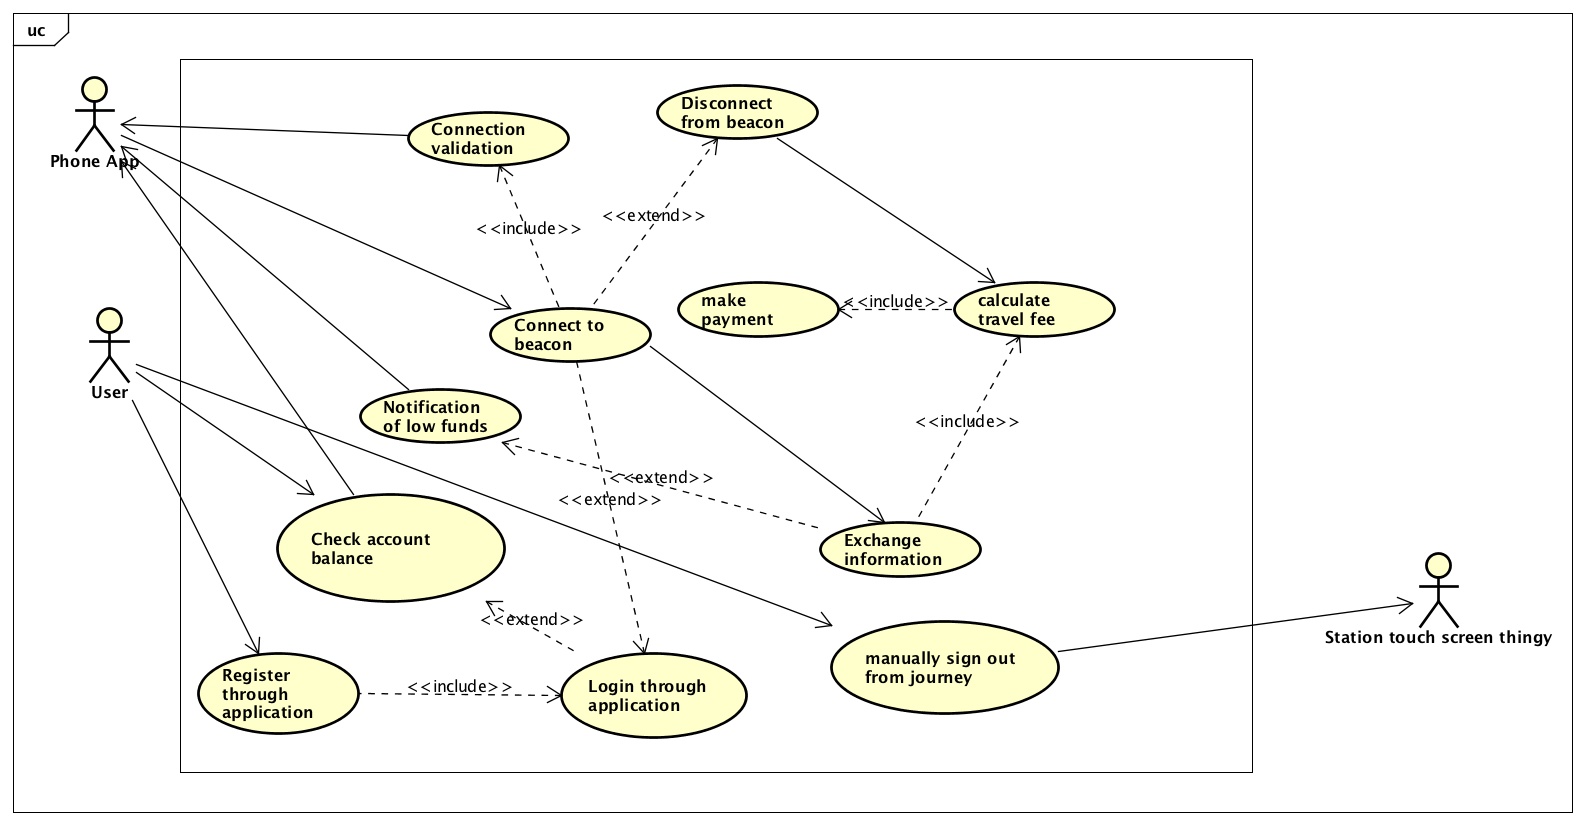
\includegraphics[width=\textwidth]{Pictures/main_use_cases.png}
	\caption{Main use cases}
	\label{fig:main_use_cases}
\end{figure}

\begin{table}[H]
	\centering
	\begin{tabularx}{\linewidth}{l|X}
		\textbf{Usecase}      & Connect phone to beacon \\ \hline
		\textbf{Main actor}  & Phone app \\ \hline
		\textbf{Goal}   & Connect to the beacon \\ \hline
		\textbf{Preconditions}     & \begin{itemize}
			\item Bluetooth is switched on
			\item App is installed
			\item Train has left the station
		\end{itemize} \\ \hline
		\textbf{Main scenario}    & \begin{itemize}
			\item The beacon discovers the phone
			\item The phone receives a notification from the beacon
			\item The beacon saves the account information locally
		\end{itemize} \\ \hline
		\textbf{Exception scenarios} & 
		\begin{itemize}
			\item The app doesn’t get the notification because
			the phone is off
			\item The app doesn’t get the notification, due to a
			communication failure 
			\item The beacon fails to detect the phone
			\item The app is installed but the owner doesn't have an account
		\end{itemize}
		\\ \hline
		\textbf{Postconditions} & 
		\begin{itemize}
			\item Phone is connected
			\item Information exchange between phone and beacon
		\end{itemize}
		
		\\ \hline
		\textbf{Related requirements} & NFR2, FR2, NFR3\\ \hline
	\end{tabularx}
	\caption{Main use cases - use case 1}
	\label{tbl:uc1}
\end{table}

\begin{table}[H]
	\centering
	\begin{tabularx}{\linewidth}{l|X}
		\textbf{Usecase}      &  Disconnect from beacon\\ \hline
		\textbf{Main actor}  & Beacon \\\hline
		\textbf{Goal}   &  Register a phone disconnection \\ \hline
		\textbf{Precondition}     &  \begin{itemize}
			\item Bluetooth is switched on
			\item Use case 1
		\end{itemize}\\ \hline
		\textbf{Main scenario}    &  \begin{itemize}
			\item The user leaves the train
			\item The beacon checks available connections
			\item The beacon sends gathered information to local server
			\item Local server sends information to main server
			\item Main server computes distance travelled by user
		\end{itemize}\\ \hline
		\textbf{Exception scenarios} & \begin{itemize}
			\item Phone battery dies before user leaves the train
			\item The beacon malfunctions and cannot check for connections
		\end{itemize}\\ \hline
		\textbf{Postconditions} & Travel distance and price are computed\\ \hline
		\textbf{Related requirements} & NFR3, FR3, FR10, FR9 \\ \hline
	\end{tabularx}
	\caption{Main use cases - use case 2}
	\label{tbl:uc2}
\end{table}

\begin{table}[H]
	\centering
	\begin{tabularx}{\linewidth}{l|X}
		\textbf{Usecase}  &  Calculate travel fee\\ \hline
		\textbf{Main actor}  & Server\\ \hline
		\textbf{Goal}   &  Charge user for travelled distance\\ \hline
		\textbf{Precondition} & \begin{itemize}
			\item Usecase 1
			\item Usecase 2
		\end{itemize} \\ \hline
		\textbf{Main scenario}  & \begin{itemize}
			\item Main server receives information regarding users which are still connected
			\item Main server compares accounts currently connected with accounts connected for previous stop
			\item Users which were connected previously and are not connected anymore are identified
			\item Travel distance and fee are calculated for identified users
		\end{itemize} \\ \hline
		\textbf{Exception scenarios} & \begin{itemize}
			\item Information cannot be transmitted between local and main servers
			\item Account is not identified
		\end{itemize}\\ \hline
		\textbf{Postconditions} & \begin{itemize}
			\item Notification regarding payment is sent to user
			\item Payment is made
		\end{itemize}\\ \hline
		\textbf{Related requirements} & FR3, FR9, FR10, FR13\\ \hline
	\end{tabularx}
	\caption{Main use cases - use case 3}
	\label{tbl:uc3}
\end{table}


\chapter{Solution strategy}
\label{chp:sol_strategy}
%!TEX root = main.tex

This chapter aims to discuss and present a concrete solution space for the problems described in chapter  \ref{chp:syst_context}. The solutions provided will directly follow the main key drivers of the project and focus on the problem space using views limited only to these most important attributes.

\section{Security}
Different security measures will be taken into account so that the information transferred between different components is not visible to external parties and remains consistent throughout the exchange.

In this manner, the security mechanisms will focus mostly on the interface levels:

\begin{itemize}
	\item \textbf{Beacon to phone:} \\
	Beacons taking part in the system will be uniquely identifiable via its id and mac address. When a phone connects to a beacon, the beacon's identity will be checked against a list of valid beacons by the mobile app. 
	
	Only if the beacon is found in the list, the connection is validated and the mobile app sends the account information to the beacon, thus keeping account information secret from external parties. 
	\item \textbf{Beacon to local server:} \\
	Similarly to the beacon verrification performed by the mobile app once a connection between the beacon and the phone is established, another verification will be performed at the level of the local server.
	
	The local server will check the identity of each beacon sending it information against a list similar to the one available to the mobile app. 
	
	As a second security mechanism, before sending information to the server, the beacons will also check the identity of above mentioned server based on a hashCode. 
	
	\item \textbf{Local to central server:} \\
	Every time the main server receives information from a local server, the identity of the local server will be checked using the hashCode mentioned for the previous connection. 
	
	Also, before sending any information to the central server, every local server will ask the central server to identify itself using a cryptographic key.
\end{itemize}


\section{Compatibility}
The compatibility of the system mainly refers to mobile phones compatibility. The system will take into consideration different types of OS and different frequencies. While not all of these possibilities are taken into consideration, the system will focuss on the most used ones:

\begin{itemize}
	\item OS compatibility(Compatibility-NF-1.1):
	\begin{itemize}
		\item Android
		\item iOS
		\item Windows
	\end{itemize}
	\item frequency: the beacons will send out 10 packages every second(Apple recommendation for optimal retrieval of packages\cite{web:beacons})
\end{itemize}

\section{Reliability}
The reliability of the system takes into consideration 3 main characteristics: availability, fault tolerance and recoverability\cite{iso}.
\begin{itemize}
	\item \textbf{Availability:} \\
	Both the local and central servers will be provided with backup servers. The information stored in the local backup servers will be updated every time the train leaves a station, while the central backup server will be updated more frequently, namely every time the central server receives information from one of the local servers. 
	
	This will allow the backup servers to be fully up to date and to minimize information loss. The backup servers will remain in a passive mode and only become functional once their corresponding main server fails to respond. Once the main server is repaired, information handling will be switched to it and the backup server will return to passive mode.
	
	Every time a main server receives information(local server from beacons and main server from local one), it will notify the senders of having received the packages through a heartbeat signal. If this signal fails to be sent, the backup server will be started.
	
	\item \textbf{Fault tolerance:} \\
	Fault tolerance will be achieved by the system using resource redundancy and duplication of information. By using the backup servers and updating their information regularly, a copy of the information will be stored at all times minimizing information loss. Also, the beacons will be placed in such a manner as to have intersecting range areas, allowing at least two beacons to monitor a specific location in the same time.
	
	\item \textbf{Recoverability:} \\
	By enabling components to keep track of received information packages, the system state is known at each point in time, which allows a very fast detection of defective components. By minimizing error detection time, the recoverability time is also minimized.
\end{itemize}



\chapter{Baseline Architecture}
\label{chp:baseline}
%!TEX root = main.tex
This chapter will provide information regarding the baseline architectural decisions taken for implementing the Easy Ticketing system. The first section will outline the main tactics used related to the key drivers and section \ref{chp:design_decisions} will describe the main architectural decisions.
 
\section{Tactics}
This section outlines the tactics used for implementing the three most important quality attributes for the system.

\subsection{Compatibility Tactics}

\subsection{Security Tactics}

Below we are briefly describing the security tactics applied for our system.
\begin{itemize} 

\item \textbf{Authenticate users}
Authentication is ensuring that a user or remote computer is actually who it purports to be.In our system (ET), every user of the mobile app needs to be authorized by inserting their personal info data. 

\item \textbf{Authorize users}
Authorization is ensuring that an authenticated user has the rights to access and modify either data or services. This is usually managed by providing some access control patterns within a system. Easy Ticketing has implemented a system, where the user will receive a notification by the time they establish a bluetooth connection with the beacon.

\item \textbf{Maintain data confidentiality} 
Data should be protected from unauthorized access. Confidentiality is usually achieved by applying some form of encryption to data and to communication links. Encryption provides extra protection to persistently maintained data beyond that available from authorization. 

\item \textbf{Maintain integrity} Data should be delivered as intended. It can have redundant information encoded in it, such as checksums or hash results, which can be encrypted either along with or independently from the original data.

\item \textbf{Limit exposure} Attacks typically depend on exploiting a single weakness to attack all data and services on a host. The architect can design the allocation of services to hosts so that limited services are available on each host.

\item \textbf{Limit access} Firewalls restrict access based on message source or destination port. Messages from unknown sources may be a form of an attack. It is not always possible to limit access to known sources. In our case Easy Ticketing  expects requests from mobile app users and from third party payment systems.  One configuration used in our case is the so-called demilitarized zone (DMZ). 
\end{itemize} 



\subsection{Reliability Tactics}

\section{Design decisions}
\label{chp:design_decisions}
%!TEX root = main.tex


\chapter{Software architecture}
\label{chp:soft_arch}
%!TEX root = main.tex


In this chapter the architecture of the system will be described. The 4+1 model will be used. We will be describing  the logical view, the physical view, the process view and the data view. 
The logical view shows the functional decomposition of the architecture into components.
the process view shows behavioral aspects of the system, the data flow view defines the data, the relation
between data entities, how the data flows through the system and the measures to ensure reliability and
performance. The physical view shows the physical entities and storage units as well as the deployment
scenario.

\section{Logical View}
This view shows the connections between structural elements, key abstractions and mechanisms that are used within SFM. At first, an overview of the components is provided. The main components of the system will be displayed in terms of layers. Next, the main components are decomposed a in term of responsibilities and interfaces.

\subsection{Primary presentation}
In order to design the software architecture of \ac{ET}, the layers pattern is used. This pattern is best suitable for the system since it gives the opportunity to abstract layers from one another, which increases the availability of the system by modularizing the components. The modularization of the components increases also the scalability and the performance of the system. 
The system has been structured according to the three-layers approach. The three main components: Mobile app, Beacon Interface and the Local Storage, and Central storage and Payment system can be seen in the figure below. 


\begin{figure}[H]
  \centering
  \includegraphics[width=\textwidth]{Pictures/arch.png}
  \caption{Overview of the System}
  \label{fig:system}
\end{figure}


\textbf{Mobile app} is the main component of our system. It will be available for download for the users and it will provide a personalized and unique account for the passengers. They can use this account to login and pay for their ticket, every time they use the trains. This layer will also enable a bluetooth connection with the beacon cart. The data collected from this layer is then sent to the other layers. 

\textbf{Beacon Interface and Local storage} This layer creates a connection with the mobile app layer. Its components are the local storage, where the data gathered from the mobile app will be stored, and the beacon interface which establishes the bluetooth connection with the mobile.

\textbf{Central Storage and Payment system} The database and the Beacon Interface are included in this layer. The data that is provided from the Mobile app layer, will be stored in the central database after the mobile phone has connected to the beacon. The calculation of the ticket fees is also done in this layer through the computational center.

\begin{figure}[H]
  \centering
  \includegraphics[width=\textwidth]{Pictures/logical.png}
  \caption{Logical View}
  \label{fig:logical}
\end{figure}

\subsection{Element Catalog}
The element catalog describes the components mentioned in the figures above.

\subsubsection{Mobile app}
The app is abstracted by the mobile app component. It is responsible for gathering the information needed by the MobileApp such as the personal info the passenger is sending. It is directly connected to the Store account info component, in order to store the data gathered by the passengers.

\subsubsection{Create account}
This component is responsible for creating the passenger's account, with all the personal data such as name, password and username regarding the passenger. This component is directly connected to the Verify account component. It first needs to verify account in order to create it.

\subsubsection{Connect Bluetooth} is another component that will handle the connection with the beacon. We can notice in the figure above that there are two Connect bluetooth components, one belonging to Mobile Application layer and the other one belonging to the Beacon Interface layer. These two components have to establish a connection in order to proceed with the ticketing. 

\subsubsection{Check-in}
This component regulates the checkin of the passenger. In order for the system to start processing the ticket fee and the journey of the passenger, it needs to connect to the beacon and to check-in, in the moment that the passenger gets in the train. 
\subsubsection{Check-out} 
The same way as the  Check-in component works, this component checks out the passenger in the moment that he/she walks out of the train. It needs to reconnect to the beacon in order to check the passenger out and to verify that the journey is finished.

\subsubsection{Store account info}
The store account info is the temporary where all the information that comes from the previous layer is stored . This is the local storage. It is directly connected to the <<Mobile app>> component, and is the first storage. It also connects to the central storage.

\subsubsection{Verify account}
Verifies that the information provided by the passengers is indeed correct and not fraud. In this component certain complex security algorithms are also implemented, in order to increase the overall security of the system and in particular to have a secure authentication of the passenger.

\subsubsection{Connect Bluetooth}
This component is strongly interconnected with the component we have mentioned above. This one belongs to the "Beacon Iterface" layer. It guarantees the connection between the phone and the beacon.

\subsubsection{Establish Bluetooth Connection} 
In order for the ticketing to succeed, it is very important for an  establishment of the bluetooth connection to happen. 

\subsubsection{Payment request} 
This component is part of the Database layer, where data is stored and processed in order to calculate the final fee. 
Firstly a payment is requested, and it is sent for authorization. Once the authorization is confirmed then the payment needs to  be calculated.

\subsubsection{Authorize payment}
This component connects to the previous one, the Payment request, in order to confirm the authorization of the payment, as it was previously mentioned. After the confirmation, this unit sends a request to the Computational unit in order to process the ticket fee.

\subsubsection{Database}
The central database stores and computes the data that is gathered from the previous layers. The central database is the main database, where everything is stored and where transactions are made. It interacts also with the third party payment system. 

\subsubsection{Authorize Account}
After the account is created it needs to be authorized. This component gets the request from the database layer. 

\subsubsection{Computational Unit}
The computational unit processes the ticket fee. It calculates the amount of the fee based on the journey of the passenger with the Calculate fee component.




\section{Process View}
This section describes the main processes performed by the system following some of the main use cases presented in chapter \ref{chp:usecases}. The following system sequence diagrams will help detail every such process by displaying the main information flows between different actors and system components in a chronological manner.

\begin{figure}[H]
	\centering
	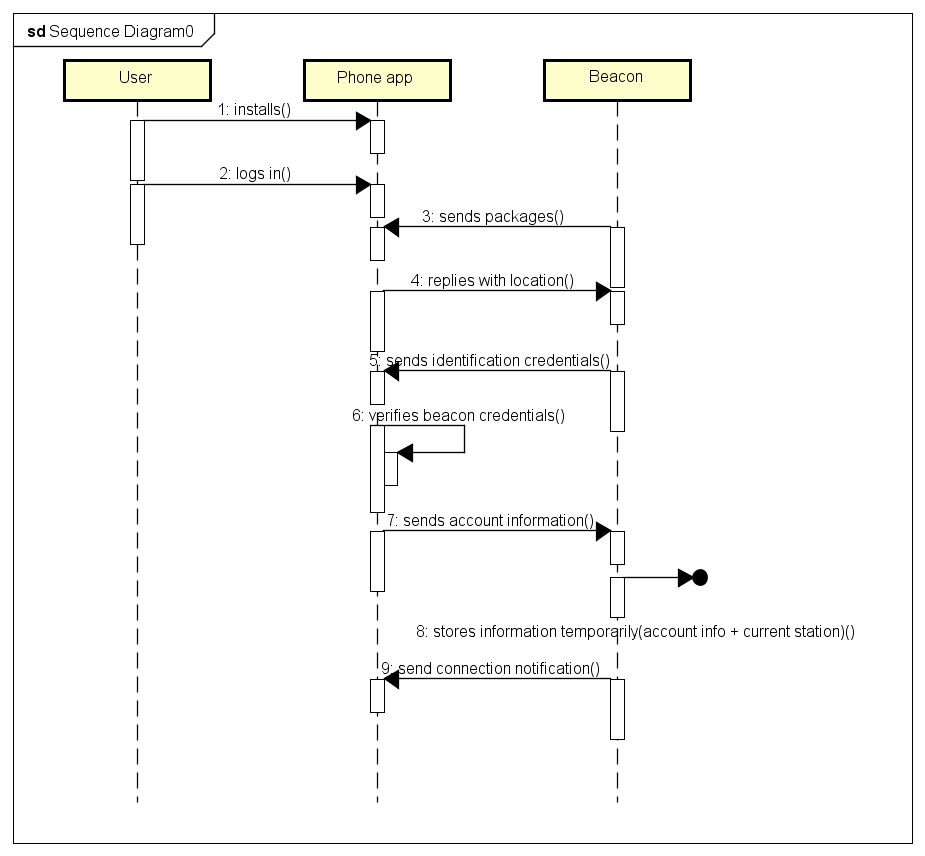
\includegraphics[width=\textwidth]{Pictures/seq_diagram_uc1.png}
	\caption{System sequence diagram- use case 1(Connect phone to beacon)}
	\label{fig:seqDiagram1}
\end{figure}
Figure \ref{fig:seqDiagram1} is a direct mapping of use case 1(connect phone to beacon).

\begin{figure}[H]
	\centering
	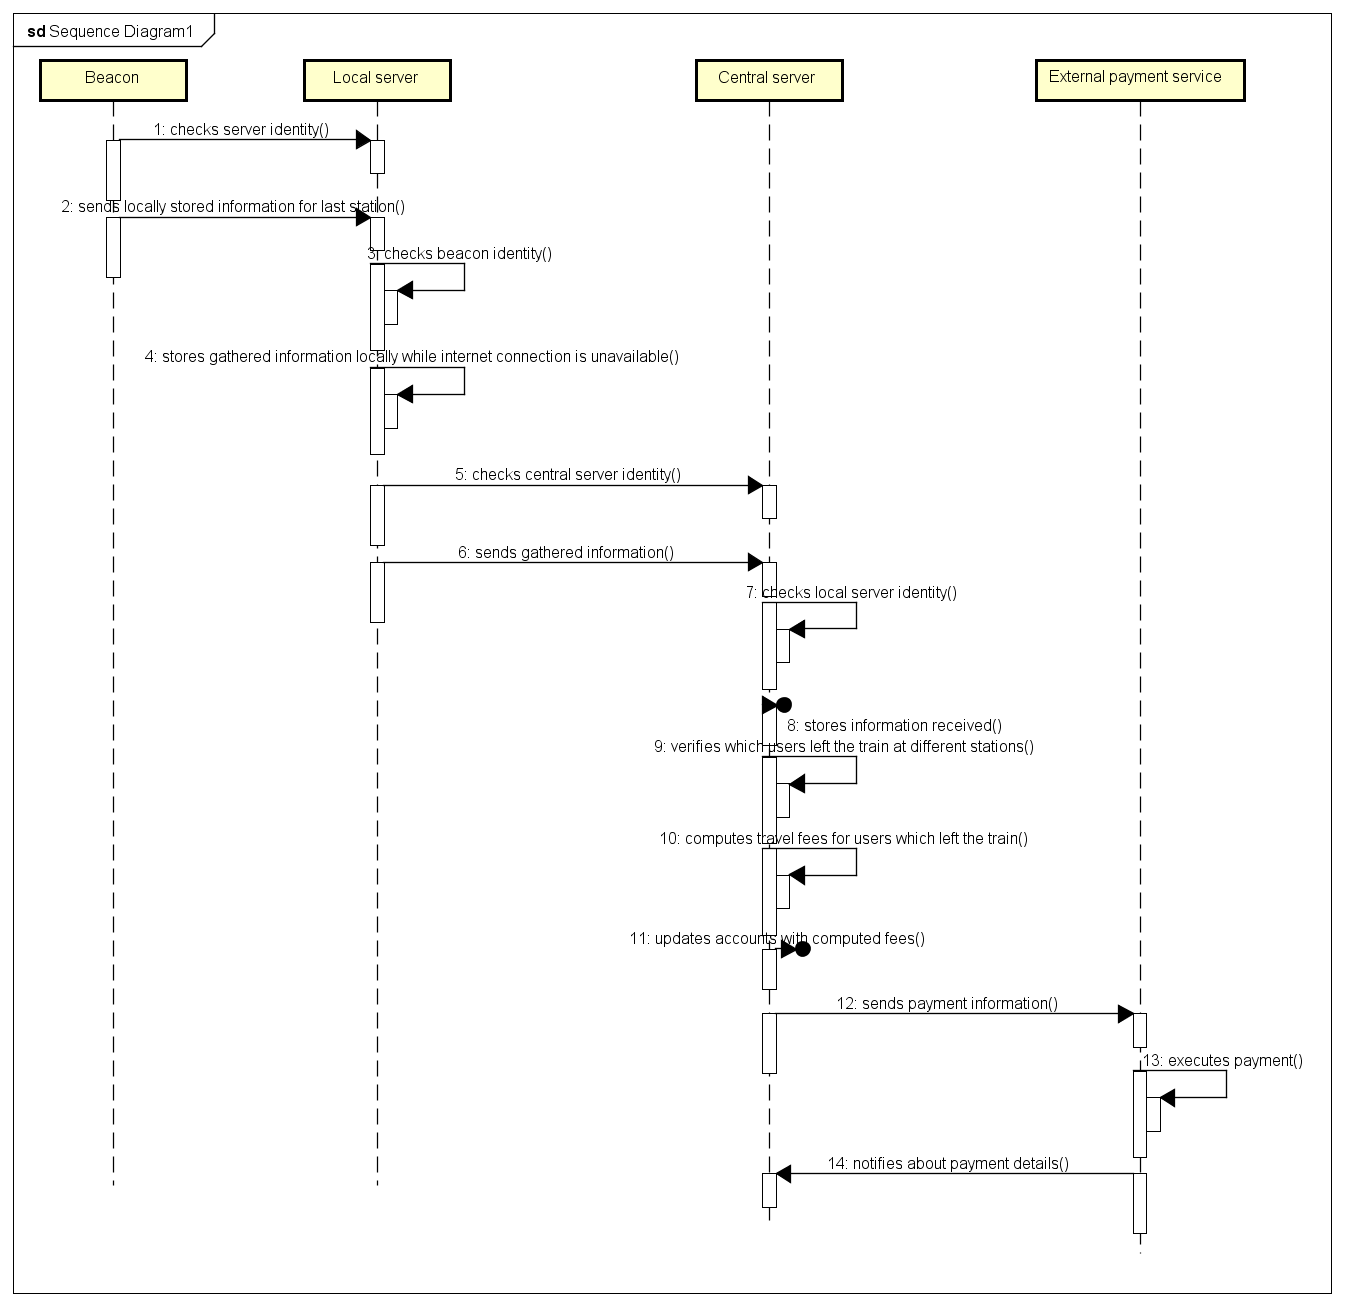
\includegraphics[width=\textwidth]{Pictures/seq_diagram_payment.png}
	\caption{System sequence diagram- payment}
	\label{fig:seqDiagram2}
\end{figure}
Figure \ref{fig:seqDiagram2} displays the information flow corresponding to use cases "Disconnect from beacon" "Calculate travel fee" and "Make payment". For this process, the system uses a third party payment service.

\begin{figure}[H]
	\centering
	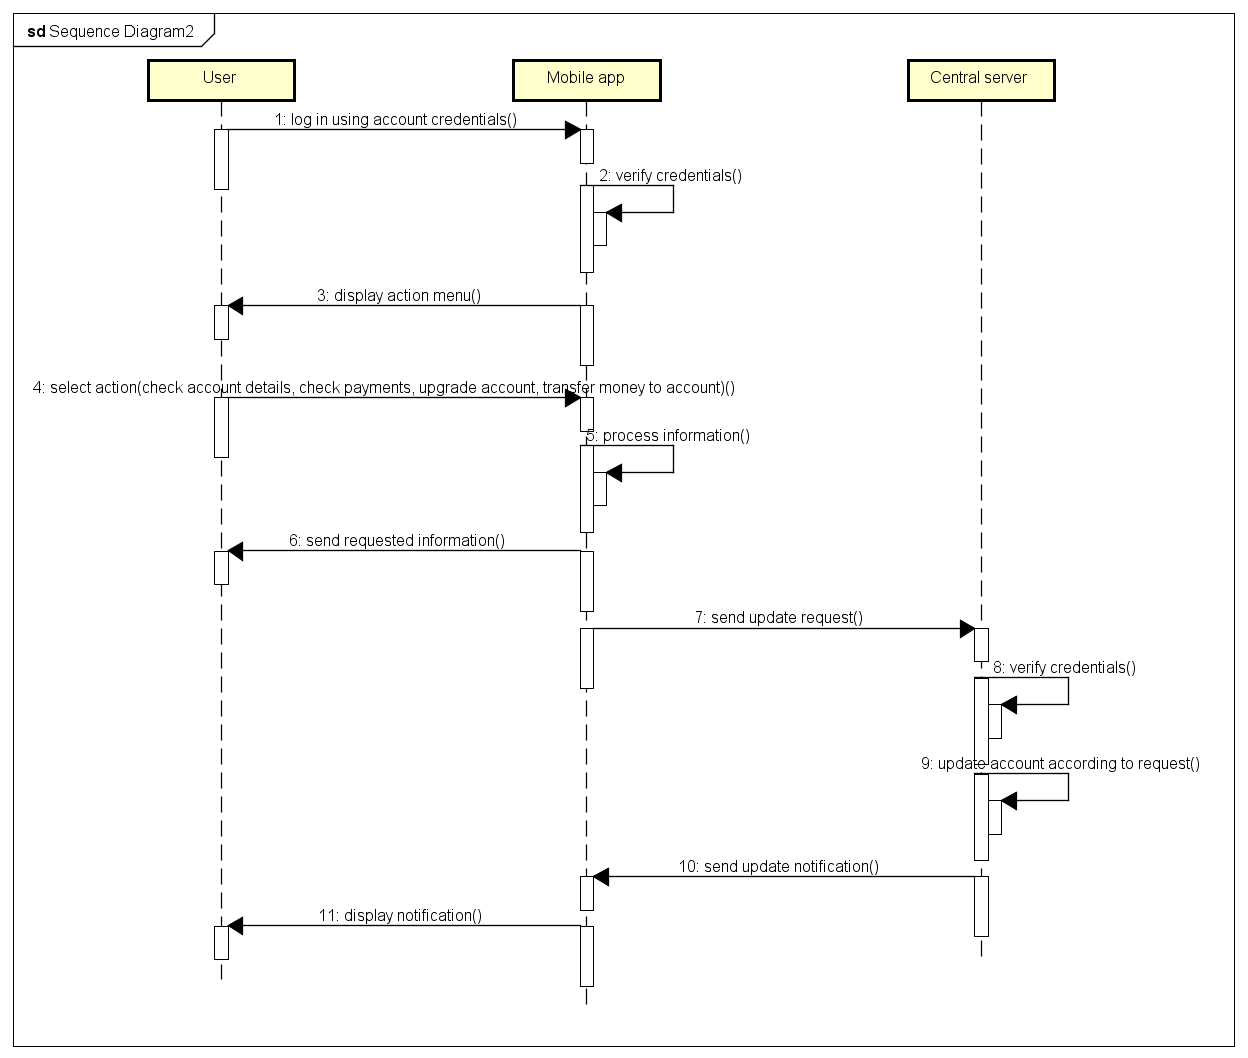
\includegraphics[width=\textwidth]{Pictures/seq_diagram_checkAccount.png}
	\caption{System sequence diagram- Check account details}
	\label{fig:seqDiagram3}
\end{figure}
Figure \ref{fig:seqDiagram3} displays the information flow related to use cases "Register through application", "Check account balance" and "Login through application". This process describes the general outline for different actions the user can perform using the mobile application.


\begin{figure}[H]
	\centering
	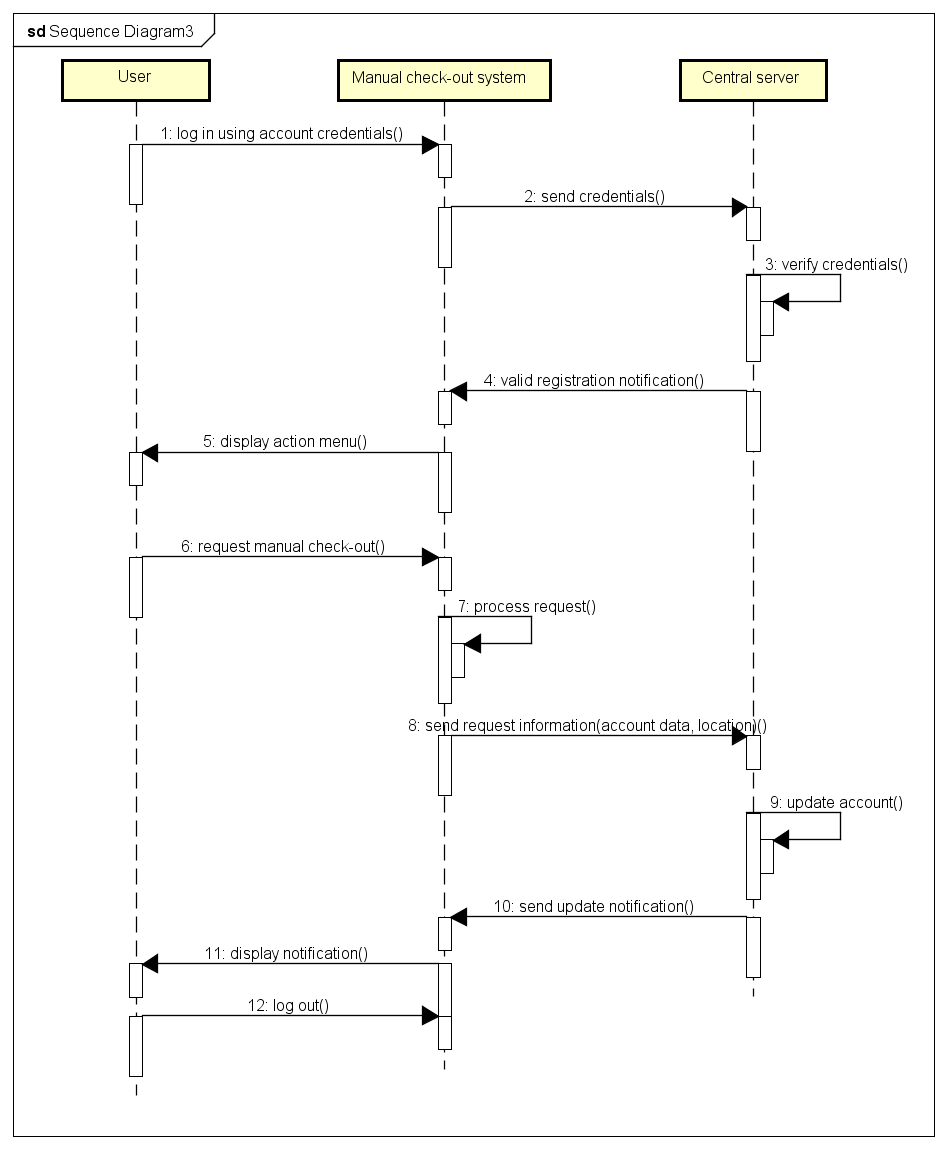
\includegraphics[width=\textwidth]{Pictures/seq_diagram_manualCheckOut.png}
	\caption{System sequence diagram- Manual checkout}
	\label{fig:seqDiagram4}
\end{figure}
Figure \ref{fig:seqDiagram4} shows the main information flow corresponding to the use case "Manually sign out from journey". This use case was designed as an alternative to the main "Disconnect from beacon" use case which will give users the possibility to manually check out at a particular train station in case of the phone to beacon connection not being available.

%\section{Data View}-- what is data view?
\section{Physical View}

\chapter{Architectural patterns}
\label{chp:patterns}
%!TEX root = main.tex




\section{Layers}



\label{subchp:layers}


%!TEX root = ../main.tex

\section{Model View Controller}
	The MVC pattern is used to break down the front-end to different pieces each providing different capabilities than the others in order to separate the representation from the logic providing it.


	\subsubsection{Source} \cite{book:design-patterns}


	\subsubsection{Problem}

		Provide an user interface which will allow for different UI capabilities used on different devices with a different purpose. Having mobile devices application which can gives more options to users and stationary units which allow users to log in and out directly at stations.

	\subsubsection{Solution} 

		Break down the UI logic in three separate pieces, namely the model , view and controller, each having one purpose only. The view is responsible with what the user will see, model with connecting to the databases and the business logic and controller with providing controlling logic and managing what view are presented thus allowing for different user interfaces for different devices based on predefined rules in the controller. 


\paragraph{Implications}
\begin{itemize}
	\item decrease performance
	\item increase modularity
	\item increase security
\end{itemize}

\label{sybchp:mvc}

%!TEX root = ../main.tex

\section{Observer Pattern}

\subsubsection{Description of pattern}

	The observer pattern is used to allow an object to publish changes to its state. Other objects subscribe to be immediately notified of any changes to the status of that particular object. 

	
\iffalse
	USAGE : The main server will observe the state of train and Activate the beacons when train leaves a station . We don't need to have the beacons active when at a station 
beacons observe when phones are in range for establishing connections
\fi

\subsubsection{Traceability} 
	% related requirements
	\begin{itemize}
		\item 1
	\end{itemize}

\subsubsection{Source} \cite{book:design-patterns}

\subsubsection{Issue} \label{observerP:issue}
	The most scalable way and also a fault-proof process for management of passengers both for current and ones who have left the train is to have the phone detection work only before and after the train has passed through a station. Having the train server to monitor beacons would make the solution highly unscalable. An operator would have to manually modify the beacons state in the train server himself. On the other hand the beacons should only have to detect nearby phones' bluetooth once or twice a transition between stations making it highly inefficient for them to be active all the time. Having the server monitor and activate all beacons and receive information about passengers would impact the performance of the solution. 

\iffalse

	Therefore there is a clash of requirements which can be solved by implementing a version of a design pattern called the Observer Pattern configured to suit the needs to both be energy efficient and fault-proof. 

	This however creates an issue that the beacons should be allowed to operate on their own and they should also monitor the state of the train.
 \fi


\subsubsection{Solution} 
	The solution to the problem listed in the \ref{observerP:issue} paragraph would be to server monitor the train and the beacons to listen to events passed through the server. The server will allow the beacons to observe its state and listen to changes in the behaviour. This could be implemented via a design pattern called Observer Pattern explained in more detail in paragraph \ref{observerP:rationale}


\subsubsection{Rationale} \label{observerP:rationale}
	Even though the Observer Design Pattern is a pattern related to coding and resolves coding issues this section look at the pattern from a different perspective. The architecture of the solution described in this document uses the Observer Pattern to allow the beacons in the train to monitor the state of the train itself. Once the train has left the station the train server will change the status to 'departed' and through attached listeners, the beacons will start their main functionality - to echo for discovered bluetooths in the particular cart they are located in.

\subsubsection{Implications}
\begin{itemize}
  \item 
\end{itemize}


\label{subchp:observerP}


\section{Replicated system}
\label{subchp:replicatedP}

%!TEX root = ../main.tex


\section{Trusted subsystem}

Trusted Subsystem : The phone needs the credentials of the beacon in order to send its credentials back to it . The beacon receives credentials from the phone and registers it in the system. 
	
\label{subchp:trustedP}


\chapter{Evaluation}
\label{chp:evaluation}
%!TEX root = ./main.tex
\section{Utility tree}
The output of the utility tree is a list of scenarios that serves as a plan
for the remainder of the ATAM evaluation. It shows the evaluation team
where the most important points are and where to examine the architectural
approaches and risks. The utility tree is composed of the key drivers of the
system, which in our case are security, reliability, and compatibility.

\begin{figure}[H]
  \centering
  \includegraphics[width=\textwidth]{Pictures/Utility-tree.png}
  \caption{Overview of the System}
  \label{fig:system}
\end{figure}

\section{Key driver verification}
In this section, we analyse and verify the patterns used for the system according to the key drivers that have been selected by the stakeholders.\\
To perform this analysis, we place the key drivers and patterns in a table and show how each key driver is affected by the selected pattern \cite{web:patterns-v-QAs} . In order to perform this analysis, a scale is used to show how much a specific key driver is affected where,
\begin{description}
\begin{itemize}
  % \item[-- --] the pattern has the worst effect on the key driver
  % \item[--] the pattern has a bad but not terrible effect
  % \item[/] the pattern's effect on the key driver is neutral
  % \item[+] the pattern has a good effect although not the best  
  % \item[++] the pattern has the best possible effect on the particular key driver
\end{itemize}
\end{description}
As a reference for some of the weightings depicted in the table, 

\begin{table}[H]
    \begin{tabularx}{\textwidth}{p{3.5cm}|>{\centering\arraybackslash}X|>{\centering\arraybackslash}X|>{\centering\arraybackslash}X}
    	 & \textbf{Security} & \textbf{Reliability} & \textbf{Compatibility} \\ \hline
    	\textbf{replicated system}         & /  & +  &  \\ \hline
    	\textbf{Model View Controller}  & /  & / &   \\ \hline
    	\textbf{layers}                    & ++ & /  &   \\ \hline
    	\textbf{trusted subsystem}         & ++ & /  &   \\ \hline
    	\textbf{master-slave replication}  & /  & ++ &   \\ \hline
	 \textbf{TOTAL} & \textbf{} & \textbf{} & \textbf{} \\
    \end{tabularx}
    \caption{Key driver verification table}
\end{table}

%\chapter{Quality scenarios}
%\label{chp:quality_scenarios}
%%!TEX root = main.tex


\listoftodos[Notes]

\appendix

\chapter{Time tracking}
\label{chp:time_track}
%!TEX root = main.tex

\begin{table}[H]
	\centering
	\begin{tabularx}{\textwidth}{p{2cm}|X|p{2.5cm}}
		\textbf{Member} & \textbf{Task} & \textbf{Time (hrs)} \\
		\hline
		ab &Introduction and goals                  & 8 \\
		   &Requirements, Key Drivers, Stakeholders & 9  \\
		   &Baseline Architecture: Security Tactics & 7  \\
		   &Software Architecture: Logical view     &12   \\
		   &Evaluation: Utility tree, scenarios     & 9  \\

		& & \textbf{45} \\
		\hline
		ph &  &  \\
			& Architectural Patterns & 22 \\
		& & \textbf{22} \\
		\hline
		am & system scope and context & 10 \\
		 & functional requirements & 3 \\
		 & solution strategy & 6 \\
		 & reliability tactics & 3 \\
		 & process view & 6 \\
		 & use cases & 7 \\
		& & \textbf{35} \\
		\hline
		er & Evaluation, Design decisions, compatibilitytactics & 21 \\
		& & \textbf{21} \\
		\hline
	\end{tabularx}
	\caption{Time tracking}
	\label{tab:timetracking-1}
\end{table}


\backmatter

\printbibliography

\end{document}
